% Para compilar la primera vez que se agrega una referencia (/cite):
% Seguir estos cuatro pasos:
% latex Nombre-del-archivo.tex
% bibtex Nombre-del-archivo (sin el .tex)
% latex Nombre-del-archivo.tex
% latex Nombre-del-archivo.tex


% Etiquetas que uso para editar en la próxima iteración:
% FALTA, VER


\chapter{ \textsc{ Diseño Digital } }\label{diseñoDigital}

\section{Introducción}
Es importante lograr sumadores binarios rápidos y eficientes según el uso de área y potencia. La suma es la operación elemental para lograr otras operaciones muy utilizadas en los circuitos aritméticos. Ejemplo de esto son los multiplicadores, la resta, división, los filtros FIR e IIR, por nombrar las más conocidas.

%FIGURA
%(Multiplicadores, Filtros FIR, usando sumadores)

Para cada una de esas operaciones, son necesarios sumadores de distinta cantidad de bits en el mismo diseño. Por lo cuál, no se trata solamente de encontrar la arquitectura que para una determinada cantidad de bits logre el mejor compromiso de área, potencia y velocidad. Sino también lograr una relación de compromiso según crece la cantidad de bits del sumador. 

\subsection{Semisumador y sumador completo}
\subsubsection{Semisumador}
El {\bf Semisumador} (Half-adder) recibe 2 bits de entradas \(a\) y \(b\) y produce un bit de suma \(s\) y un bit de acarreo \(c\).

\begin{subequations}
\begin{align}
s &= a \oplus b\\
c &= ab
\end{align}
\end{subequations}

\subsubsection{Sumador Completo}
Luego definimos un Sumador Completo de un bit, o Full Adder:
\begin{center}
\begin{tabular}{lll}
Entradas: & Bits de operandos \(a\) , \(b\) y carry-in \(c_{in}\) & (o \(a_i, b_i, c_i\) para la etapa \(i\)) \\
Salidas: & Suma \(s\) y carry-out \(c_{out}\) & (o \(s_i\) y \(c_{i+1}\) para la etapa \(i\)) \\
\end{tabular}
\end{center}

\begin{subequations}
\begin{align}
s &= a\oplus b \oplus c_{in}
\label{s}
\\
c_{out}&= a b + a c_{in} + b c_{in}
\label{c}
\end{align}
\end{subequations}
%\(c_{out}= (a\wedge b )\vee (a \wedge c_{in}) \vee (b\wedge c_{in})\)

Podemos construir un {\bf sumador completo} (full-adder) combinando las ecuaciones del sumador y semisumador, como vemos en la figura \ref{fig:fulladder}:

\vspace{-1pt}

\begin{figure}[h]
  \centering
\hspace{-23pt}
\begin{subfigure}[b]{0.3\textwidth}
                \centering
                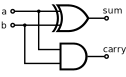
\includegraphics[width=\textwidth]{figuras/halfadd_schem.pdf}
                \caption{Semisumador}
                \label{fig:halfadder}
        \end{subfigure}
\begin{subfigure}[b]{0.5\textwidth}
                \centering
                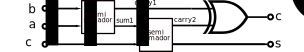
\includegraphics[scale=1.3]{figuras/fullAdd_schem.pdf}
                \caption{Sumador completo}
                \label{fig:fulladder}
        \end{subfigure}

  \caption{Bit adders}\label{fig:bitadders}

\end{figure}

\vspace{0.5cm}



\section{Selección de la arquitectura del sumador}

Proponemos el uso de Celdas estándard CMOS (Complementary Metal Oxide Silicon) para la implementación\footnote{Para ver otras posibilidades de implementación lógica, ver (FALTA CITA) RABAEY}. El carácter de nuestro flujo de diseño así lo requiere, ya que se utilizarán herramientas de síntesis de circuitos digitales basadas en celdas estándars. Quedan entonces descartadas las implementaciones utilizando transmition gates, lógica dinámica u otro tipo de implementacion lógica.

\subsection{Costo, Retardo y Área de los circuitos combinacionales}
Cada circuito combinacional \(G\) tiene un costo, área y un retardo. El costo de un circuito combinacional es la suma de los costos de las compuertas en un circuito. Le asignamos un costo unitario a cada compuerta, y el costo del circuito combinacional \(c(G)\) es igual al número de compuertas en el circuito.

El retardo de un circuito combinacional \(d(G)\) se define igual al del retardo de una compuerta. Es el menor tiempo requerido para que las salidas se estabilicen, asumiendo que todas las entradas están estables. Para simplificar el análisis, se le asigna un retardo unitario a cada compuerta.

El área de un combinacional se compone por el area total (\emph{cell area}) de las compuertas utilizadas mas el área total de todas las conexiones (\emph{net area}). 

\subsection{Clasificación de los sumadores}

Dentro de los sumadores paralelos, se encuentran varias arquitecturas, cada una con sus ventajas y desventajas. Hacemos una lista de algunas de ellas:

\vspace{0.3cm}

\begin{tabular}{ |l|l| }
  \hline
  \multicolumn{2}{|c|}{Sumadores Binarios} \\
  \hline

RCA & Ripple Carry Adder \\
CLA & Carry Look-Ahead Adder \\
CSkA & Carry Skeep Adder \\
CA & Canonical Adders \\
BBCLA & Block-based Look-Ahead Adders \\
CondSumA & Conditional Sum Adder \\
CSeA & Carry Select Adder \\
HybAd & Hybrid Adders \\
NPA & Network Prefixs Adders: \\
& Ladner and Fischer \\
&Kogge-Stone \\
&Brent-Kung \\
&Skalansky \\
  \hline
\end{tabular}
\vspace{0.3cm}

%Carry Save Adder (CSaA) & \(O(n) \)& \(O(\log (n)) \)\\ \hline
%Carry Skip Adder (CSA) &\( O(n) \)& \(O(n^{l+2/l+1})\) \\ \hline
%Carry Increment Adder (CIA) &\( O(n)\) &\( O(n^{l+2/l+1})\) \\ \hline

\subsubsection{Ripple Carry Adder}

Definimos el sumador Ripple Carry Adder (RCA), utilizando \(n\) sumadores completos para sumar 2 operandos de \(n\) bits. El sumador de \(n\) bits produce una salida de \(n\) bits y una salida de acarreo \(c_{out}\)

Este sumador se implementa conectando como muestra la figura \ref{fig:RCA} el bloque \verb.fullAdd. (Sumador Completo). El camino crítico de la señal se determina considerando el peor camino de propagación de la señal.  

%\vspace{-1pt}
\begin{figure}[h]
  \centering
\includegraphics[scale=1.5]{figuras/binnaryAdder.pdf}
  \caption{Ripple Carry Adder}
  \label{fig:RCA}
\end{figure}

El retardo del camino crítico de un sumador de $n$ bits es:

\begin{equation}
T_{RCA} = (n-1)T_m+ T_{FA}$
\end{equation}

Siendo $T_m$ el retardo del circuito de generación del acarreo de un sumador completo y $T_{FA}$ el retardo de un sumador completo. Es decir, el retardo es proporcional al tamaño de los operandos.

%\cite{estrada-gimenez}
%Comenzamos con el RCA (Ripple Carry Adder), que tiene un área O(n) y un retardo de compuerta (Delay) de O(n).
%Luego tenemos al CLA (Carry Look-Ahead Adder) con un área de O(n*log(n)) y un delay de O(log(n)).
%Carry Skip Adder(CSA)
%Carry Increment Adder (CIA) Área O(n) y Delay O (nl + 2/ l +1 )  
%Carry Select Adder (CSelA)Área O(n) y Delay O (nl + 2/ l +1 ) 
 
% El delay de un RCA está en pag. 77 de Computer Arithmetic de Behrooz Parhami

\subsection{Carry Lookahead Adders}

La clave para sumar rápido es plantear el problema de la suma como el problema de generar las señales de acarreo en el menor tiempo posible; eso queda evidenciado al interpretar la ecuación \ref{s_i}. Por lo tanto, el objetivo será lograr un bloque generador de las señales de acarreo de baja latencia\cite{arithmeticComputer}.
%Pag. 85 - Section 5.6 (ver como se cita en latex la página)

Ya que una vez que el acarreo en la posición \(i\) es conocido, se puede calcular la suma como:
\begin{equation}
s_i = a_i \oplus b_i\oplus c_i\label{s_i}
\end{equation}

Con respecto al acarreo, lo importante es si en una posición dada el acarreo se \emph{genera} ó se \emph{propaga}. Con las siguientes ecuaciones lógicas podemos definir esas señales:
%

%\vee es el OR
%\wedge es el AND
%\oplus es el XOR
%$$a_i=\lnot{a_i}\wedge\lnot{b_i}=\lnot{(a_i \vee b_i)}$$
$$g_i=a_ib_i$$
$$p_i=a_i \oplus b_i$$


Asumiendo que estas señales se han calculado y están disponibles, podemos calcular recursivamente el acarreo de la siguiente forma:
\begin{equation}
%c_{i+1}=g_i\vee (c_i \wedge p_i)
c_{i+1}=g_i + c_i p_i
\end{equation}


\noindent quiere decir que un acarreo entrará en una etapa \(i+1\) si este se genera en la etapa \(i\) ó entra en la etapa \(i\) y se propaga en esa etapa.

\subsection{Desenrollando la recurrencia del acarreo}
Uno puede desenrollar esta fórmula recursiva del acarreo hasta lograr una función que dependa directamente de los operandos ($a$ y $b$) y del acarreo de entrada $c_{\text{in}}$:
\begin{equation}
\begin{align}
c_i &= g_{i-1} + p_{i-1}c_{i-1}\notag\\
&=g_{i-1}+p_{i-1}(g_{i-2}+p_{i-2}c_{i-2})=g_{i-1}+p_{i-1}g_{i-2}+p_{i-1}p_{i-2}c_{i-2}\notag\\
&=g_{i-1} + p_{i-1}g_{i-2}+p_{i-1}p_{i-2}g_{i-3}+p_{i-1}p_{i-2}p_{i-3}c_{i-3}\notag\\
&=g_{i-1} +p_{i-1}g_{i-2}+p_{i-1}p_{i-2}g_{i-3}+p_{i-1}p_{i-2}p_{i-3}g_{i-4}+p_{i-1}p_{i-2}p_{i-3}p_{i-4}c_{i-4}\label{gyp}	
\end{align}
\end{equation}

El proceso se repite hasta que el último término contenga $c_0 = c_{\text{in}}$. Podemos computar todos los acarreos en un sumador de $k$-bit directamente con las señales auxiliares ($g_i,p_i$) y $c_{\text{in}}$, utilizando compuertas lógicas AND-OR con un fan-in máximo de $k+1$. Para $k=4$, tenemos:
\begin{equation}
\begin{align}
c_4 &=g_{3} +p_{3}g_{2}+p_{3}p_{2}g_{1}+p_{3}p_{2}p_{1}g_{0}+p_{3}p_{2}p_{1}p_{0}c_{0}\\
c_3 &=g_{2} +p_{2}g_{1}+p_{2}p_{1}g_{0}+p_2p_1p_0c_0\\
c_2 &=g_{1} +p_{1}g_{0}+p_{1}p_{0}c_{0}\\
c_1 &=g_0+p_0c_0\\
\label{carries}	
\end{align}
\end{equation}	
Aquí, $c_4$ y $c_0$ son los $c_{\text{out}}$ y $c_{\text{in}}$ respectivamente de un sumador de 4-bits. Podemos usar un bloque de acarreo basado en estas ecuaciones, y usando compuertas AND de 2 entradas para $g_i$ y compuertas XOR de 2 entradas para $p_i$ y los bits de suma, construimos un sumador de 4-bits. Este sumador es conocido como \emph{carry lookahead adder (CLA)}. Notar que como $c_4$ no se usa para calcular la suma, lo podemos obtener usando una ecuación mas simple:
\begin{equation}
\begin{align}
c_4 = g_3 + c_3p_3 \notag
\end{align}
\end{equation}
Sin tener casi un deterioro en velocidad. La red de acarreo que resulta de estas ecuaciones la podemos ver en la figura \ref{cla4bits}.
\begin{figure}[h]
  \centering
\includegraphics[scale=0.43]{figuras/fulladder4bitcla.png}
\vspace{-1pt}
  \caption{CLA 4-bits}
  \label{cla4bits}
\vspace{-15pt}
\end{figure}

Si observamos las ecuaciones \ref{carries}, vemos que el retardo de esta red será el retardo $T_{AND_n}$ de la mayor celda AND, mas el retardo $T_{OR_n}$ de la operación OR de $n$ entradas. Esto es un inconveniente, ya que según aumenta el fan-in también aumenta el retardo. El retardo de un sumador construido con esta red tendrá también el retardo $T_p$ del cálculo de $p$ mas el retardo de un sumador completo.
\begin{equation}
T_{CLA} = T_p + T_{AND_n} + T_{OR_n} + T_{FA}
\end{equation}

Se pueden realizar por medio de árboles binarios una reducción a celdas con un fan-in de dos (por ejemplo), pero agregando una etapa por cada reducción, en ese caso el retardo en este circuito sería en función del $\log_2 n$.


%\subsection{Lower Bounds}
%Teorema:
%Si el número de entradas de cada compuerta combinacional está acotado por c, entonces para cada circuito %combinacional \(G\) que implemente un \(sumador(n)\), se da que:

%\(c(G) \greatereq n/c \) and \(d(G) \greatereq \log_{c}(n)\)

% INTERESANTE: Clock periods in contemporary microprocessors are rather short; they are shorter than 10 times the delay of a full-adder.

\subsection{Sumadores de Prefijo Paralelos (\emph{Parallel Prefix Adders})}
En la sección anterior vimos como desarrollar ecuaciones que nos permiten obtener las señales de acarreo a partir de las señales auxiliares, para poder calcular la suma del bit $n$, sin esperar a que el acarreo del bit $n-1$ sea computado. Aunque esta solución tal cuál como la presentamos deja de ser aplicable según aumenta $n$, nos permite abordar el problema del cálculo de los acarreos como un problema de prefijos paralelos.
\subsubsection{Problema de Prefijos Paralelos (\emph{Parallel Prefix Problem})}
El problema de prefijo paralelo es:

\begin{equation}
\begin{align}
\text{Dado:}\\
 & \text{Entradas:} x_0,x_1,\dotsc,x_{k-1} \\
 & \text{Un operador + asociativo}\\ 
\text{Computar}:&x_0 \nonumber \\
&x_0+x_1 \nonumber \\ 
&x_0+x_1+x_2+ \nonumber \\ 
&\vdots \nonumber \\ 
&x_0+x_1+x_2+\dotsb+x_{k-1} \nonumber
\end{align}
\end{equation}

\subsubsection{Cómputo del acarreo como un problema de prefijo paralelo}
Pensemos la ecuación \ref{gyp} de la siguiente forma, asumiendo que $c_0=c_\text{in}$ viene desde otro bloque:
\begin{equation}
\begin{align}
g_{[i,i+3]} &= g_{i+3}+g_{i+2}p_{i+3}+g_{i+1}p_{i+2}p_{i+3}+g_{i}p_{i+1}p_{i+2}p_{i+3}\nonumber\\
p_{[i,i+3]} &= p_{i}p_{i+1}p_{i+2}p_{i+3}\nonumber
\end{align}
\end{equation}

Podemos interpretar estas ecuaciones de la siguiente forma: las cuatro posiciones de bits propagan colectivamente un acarreo $c_\text{in}$ si y solo sí cada una de las posiciones propaga; y el bloque genera un acarreo si en la posición $i+3$ se genera uno, o se podrouce en la posición $i+2$ y es propagado por la posición $i+3$, etc.

Con este procedimiento podemos llegar a expresar una generalización muy importante, para bloques adyacentes que se superponen $[i_1,j_i]$ y $[i_0,j_0]$, con $i_0 \leq i_1 - 1 \leq j_0 < j_i $:
\begin{equation}
\begin{align}
g_{[i_0,j_1]} &= g_{[i_1,j_1]}+g_{[i_0,j_0]}p_{[i_1,j_1]} \nonumber\\
p_{[i_0,i_1]} &= p_{[i_0,j_0]}p_{[i_1,j_1]}\nonumber
\end{align}
\end{equation}
Aquí, $g_{[i_0,j_1]}$ y $p_{[i_0,i_1]}$ son las señales que producimos de 2 bloques adyacentes ($B''$ y $B'$ con sus señales asociadas $(g'',p'')$ y $(g',p')$) que para simplificar la notación nos permite reescribir la anterior ecuación como:
\begin{equation}
\begin{align}
g &= g'' + g'p''\nonumber\\
p &= p'p''\nonumber
\end{align}
\end{equation}
Ahora entonces definimos un operador acarreo $\circ$ para condensar estas operaciones:
\begin{equation}
\begin{align}
(g,p) &= (g'',p'') \circ (g',p') = (g'' + g'p', p'p'')\nonumber
\end{align}
\end{equation}
Este operador es un operador asociativo, y esto se puede demostrar utilizando la propiedad asociativa de los operadores OR y AND. Finalmente, ya tenemos un operador asociativo, y las entradas $(g''',p''')$,$(g'',p'')$,$(g',p'),\ldots$ que nos permiten plantea el problema de la construcción de la red (o bloque) de acarreos, como un problema de \emph{Prefijos Paralelos}:

\begin{equation}
\begin{align}
\text{Dados:}\\
 & \text{Entradas:} (g_0,p_0),(g_1,p_1),\dotsc,(g_{k-1},p_{k-1}) \\
 & \text{Un operador} \circ \text{asociativo}\\ 
\text{Computar}:
(G_0,P_0) = &(g_{[0,0]},p_{[0,0]})\notag\\
(G_1,P_1) = &(g_{[0,0]},p_{[0,0]})\circ(g_{[0,1]},p_{[0,1]})\notag\\
&\vdots \nonumber \\
(G_{k-1},P_{k-1}) = &(g_{[0,0]},p_{[0,0]})\circ(g_{[0,1]},p_{[0,1]})\circ \dotsc \circ(g_{[0,k-2]},p_{[0,k-2]})\circ(g_{[0,k-1]},p_{[0,k-1]})\notag
\end{align}
\end{equation}
Retomando la ecuación \ref{s_i} de la suma, y con estas ecuaciones que nos dan las señales propagadas o generadas del acarreo, podemos construir distintos sumadores, que varían en la red de cálculo del acarreo, particularmente en cómo se elija la asociación del operador punto. La implementación mas básica (y lenta) sería la de ir asociando en serie a este operador.  
%Seria interesante hacer el gráfico de la red serial de acarreo.

PORHACER: AGREGAR GRAFICO DE UNA RED SERIE

%118 del Parhami " Computer Arithmetic: Algorithms and Hardware Designs."

\subsection{Selección de la arquitectura}

Se puede afirmar que los llamados sumadores paralelos prefijo son mejores con respecto al producto Potencia - Retardo. Aunque no hay una estructura que pueda calificarse como globalmente la mejor. Estos sumadores reducen el problema de calcular de forma paralela las señales de acarreo como el problema de un cálculo de prefijo.


Brent Kung\cite{brent-kung}, Kogge Stone \cite{kogge-stone}, Ladner Fisher [3], Hans Carlson\cite{kogge-stone} y Knowles\cite{knowles} son implementaciones que se diferencian en que cada caso por minimizar alguna relación de compromiso, en el espacio de diseño para minimizar retardo, area y potencia. Por ejemplo citamos un estudio que presenta los siguientes resultados de la figuras \ref{retardo-bits} y \ref{area-bits} de un estudio comparativo \cite{estrada-gimenez} para tecnología CMOS 0,13~$\mu$m.

\begin{figure}[h]
  \centering
\includegraphics[scale=0.34]{figuras/retardo-bits.png}
\vspace{-5pt}
  \caption{Retardo respecto al tamaño de los operandos}s
  \label{retardo-bits}
\vspace{-5pt}
\end{figure}


\begin{figure}[h]
  \centering
\includegraphics[scale=0.34]{figuras/area-bits.png}
\vspace{-1pt}
  \caption{Área respecto al tamaño de los operandos}
  \label{area-bits}
\vspace{-15pt}
\end{figure}

\begin{table}[t]
\caption{Resumen Características de Sumadores}
\centering
\begin{tabular}{|l|l|l|}
\hline
\multicolumn{1}{|c|}{\textbf{Arquitectura}} & \multicolumn{1}{c|}{\textbf{Retardo Máx.   }} & \multicolumn{1}{c|}{\textbf{Área}} \\ \hline
Ripple Carry Adder (RCA) & \(O(n)\) & \(O(n)\) \\ \hline
Carry Save Adder (CSaA) & \(O(\log(n)) \)& \(O(n) \)\\ \hline
Carry Look-Ahead Adder (CLA) & \(O(\log(n))\) & \(O(n\log(n))\) \\ \hline
Carry Skip Adder (CSA) &\(O(n^{l+2/l+1})  \)& \(O(n)\) \\ \hline
Carry Increment Adder (CIA) &\(O(n^{l+2/l+1})  \)& \(O(n)\) \\ \hline
Carry Select Adder (CselA) &\(O(n^{l+2/l+1})  \)& \(O(n)\) \\ \hline
Ladner-Fisher &\( O(\log_2(n))\) & \(O(n\log(n))   \) \\ \hline
Skalansky &\( O(\log_2(n))\) & \(O(\log^2(n))\) \\ \hline
Kogge-Stone & \( O(\log_2(n))\) & \\ \hline
Han-Carlson &Falta &Falta \\ \hline 
Brent-Kung & \(O(\log_2(n))\ & \(O(n\log_2(n))\) \\ \hline

\end{tabular}
\label{sumadores}
\end{table}
Resumimos en la tabla \ref{sumadores} las características y diferencias entre los distintos sumadores\cite{6120598}.

%Agregar las referencias a los papers si se puede

%Para justificar la tabla de arriba, vemos los siguientes dos papers:

%"A unified Adder Design" - Wang, Parhi.

%CARACTERIZACIÓN DE SUMADORES EN TECNOLOGÍAS FUERTEMENTE SUBMICRÓNICAS -  Adrián Estrada, Carlos J. Jiménez, Manuel Valencia

\subsubsection {Sumador Rápido de Brent-Kung}
Para para tener en cuenta el problema de la interconexión entre las compuertas de forma tal que estas sean mínimas y que el área de celdas y de conexión se minimicen, se propone el sumador de Brent-Kung. Este sumador \cite{brent-kung} es una versión que considera el problema de la interconexión entre las compuertas, de una forma que minimice el área, a costa de un aumento en el retardo. Esto se expresa en la función de retardo que es \(2\log_2(n)-2\), a diferencia de los sumadores de Ladner-Fisher\cite{ladner-fischer} y Kugge-Stone\cite{kogge-stone} que en \(\log_2(n)\) etapas calculan todos las señales de acarreo. 


\subsubsection {Operador de Brent-Kung}
El operador $\circ$ se define\footnote{ Para respetar la notación de la bibliografía original comenzamos a utilizar la notación lógica con \(\vee\), \(\wedge\) y \(\oplus\) como los operadores booleanos AND, OR y XOR respectivamente} como:
\begin{equation}
(g,p) \circ (\hat{g},\hat{p}) = (g\vee(p\wedge\hat{g}),p\wedge\hat{g})\label{gap}\end{equation}


\begin{figure}[h!]
  \centering
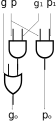
\includegraphics[scale=1.0]{figuras/dotOp_schem.pdf}
\vspace{-5pt}
  \caption{Operator Punto de Brent-Kung}
  \label{dotOp}
\vspace{-15pt}
\end{figure}
El operador Punto de Brent-Kung es asociativo, es decir:
$$((a,b) \circ( c,d))\circ (e,f)  = (a,b)\circ((c,d)\circ(e,f))$$
Y por lo tanto podemos ahorrarnos los paréntesis y escribimos:
$$(a,b)\circ(c,d)\circ(e,f)\circ...$$

\subsubsection {Circuito de Generación y Propagación de acarreo}
Ahora necesitamos un circuito que con cada bit de entrada de los operandos \(a\) y \(b\) calcule la señal de acarreo y la de propagación:
$$g_i=a_i \wedge b_i, p_i=a_i\oplus b_i$$
Esas señales se generan en paralelo, dado dos números binarios \(a[n]\) and \(b[n]\) de longitud \(n\).

%vspace{-10pt}

\begin{figure}[h!]
  \centering
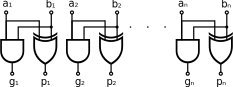
\includegraphics[scale=1]{figuras/gAndPs_schem.pdf}
%\vspace{-5pt}
  \caption{Generación y Propagación del Acarreo}
  \label{gAndPs}
%\vspace{-5pt}
\end{figure}

\subsubsection {Circuito completo}
Asumiendo que ya tenemos diseñado el bloque de cálculo de los acarreos en cadena, al cual le llamamos red de prefijos paralelos, el circuito propuesto por el paper de Brent-Kung\cite{brent-kung} lo podemos ver como en la figura \ref{bkungadder}, que nos servirá a la hora de la implementación en HDL.

\begin{figure}[h]
  \centering
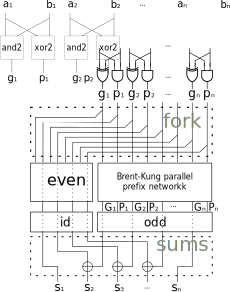
\includegraphics[scale=1.5]{figuras/arquitectura_schem.pdf}
  \caption{Sumador de Brent-Kung}
  \label{bkungadder}
\end{figure}

\subsubsection {Red de Prefijos Paralelos}
\noindent Con la figura \ref{bKung16}, detallamos ahora la red de prefijos paralelos con un fan-out máximo de dos, lo cuál diferencia a el sumador de Brent-Kung de los otros sumadores de prefijos paralelos. La red se realiza con 2 elementos: Los puntos negros son los operadores punto de Brent-Kung de la figura \ref{dotOp} y con buffers (los puntos blancos) que realizan una copia de la señal. Cada cable representa un par de bit \(g_i\),\(p_i\) de la figura \ref{bkungadder}.


\begin{figure}[h!]
\vspace{-5pt}
  \centering
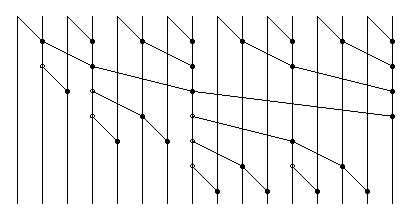
\includegraphics[scale=1.4]{figuras/bKung16.eps}
  \caption{Red de prefijos paralelos (ejemplo de 16 bits)}
\label{bKung16}
\vspace{-10pt}
\end{figure}

\section{Implementación en Lenguaje de Descripción de Hardware}
Ya hemos presentado una descripción esquemática del sumador binario de \(n\) bits. El objetivo es implementar el circuito en un lenguaje de HDL parametrizado por el tamaño \(n\) del los números binarios a ser sumados. Para describir el circuito, elegimos Lava, un sistema para diseñar, especificar, verificar e implementar hardware. Lava está embebido en el lenguaje de programación funcional Haskell. En lava los circuitos son descriptos como funciones que operan sobre listas, tuplas o sobre circuitos. Esto último se debe que el lenguaje Haskell permite la definición de funciones de alto orden, es decir podemos definir funciones que su dominio e imagen son funciones. 

\subsection{Implementación del RCA en lava}

\noindent Siguiendo la figura \ref{fig:halfadder}, definiremos el semisumador:
\begin{lstlisting}
halfAdd (a, b) = (s, c)
   where
      s = xor2 (a, b)
      c = and2 (a, b)
\end{lstlisting}
\noindent Para escribir el circuito del sumador completo usamos la figura \ref{fig:fulladder}, nombrando las señales internas y escribiendo los subcomponentes de la siguiente forma:
\begin{lstlisting}
fullAdd (cin, (a, b)) = (s, cout)
    where
       (sum1, carry1) = halfAdd (a, b)
       (s   , carry2) = halfAdd (cin, sum1)
       cout           = xor2 (carry2, carry1)
\end{lstlisting}

Por último escribimos la descripción del sumador binario (RCA) de la figura \ref{fig:RCA} de la siguiente forma:

\begin{lstlisting}
adder (carryIn, ([], []))     = ([], carryIn)
adder (carryIn, (a:as, b:bs)) = (sum:sums, carryOut)
   where
      (sum, carry)     = fullAdd (carryIn,(a, b))
      (sums, carryOut) = adder (carry, (as, bs))
\end{lstlisting}

\subsection{Patrones de conexión}
\paragraph{Patrones de conexión estandars.} Los patrones de conexión son funciones de alto orden\footnote{Las funciones de alto orden (\emph{high order functions}) son funciones que toman otras funciones como argumento y devuelven otra función como resultado.} que pueden ser utilizadas para construir circuitos, les llamamos circuitos de alto orden o generadores de circuitos.

\begin{figure}[h]
  \centering
\hspace{-23pt}
%[width=\textwidth]
\begin{subfigure}[b]{0.45\textwidth}
                \centering
                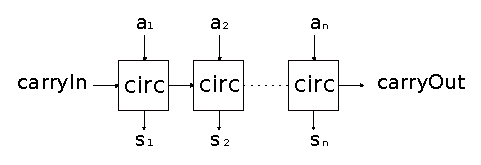
\includegraphics[scale=0.9]{figuras/rowCirc.eps}
                \caption{row}
                \label{fig:rowcirc}
        \end{subfigure}
\begin{subfigure}[b]{0.25\textwidth}
                \centering
                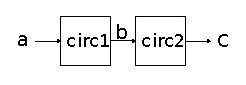
\includegraphics[scale=1]{figuras/serial.eps}
                \caption{serial}
                \label{fig:serial}
        \end{subfigure}
\begin{subfigure}[b]{0.30\textwidth}
                \centering
                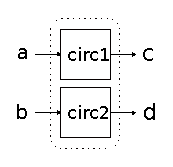
\includegraphics[scale=1]{figuras/par.eps}
                \caption{parallel}
                \label{fig:parallel}
        \end{subfigure}
  \caption{Diferentes Patrones de Conexión de Circuitos}\label{fig:pattern}
\end{figure}


Observando la definición de {\footnotesize\verb|adder|} y su topología, podemos generalizar esa estructura de conexión reemplazando el circuito por un parámetro, que en la definición\footnote{Esto es posible dado que Haskell implementa \emph{pattern matching}.} del circuito será una entrada mas. A ese parámetro lo nombramos {\footnotesize\verb|circ|}:

\begin{lstlisting}
row circ (carryIn, ([])) = ([], carryIn)
row circ (carryIn, a:as) = (b:bs, carryOut)
   where
      (b, carry)     = circ (carryIn, a)
      (bs, carryOut) = row circ (carry, as)
\end{lstlisting}
\end{figure}
La función {\footnotesize\verb|row|} toma un circuito {\footnotesize\verb|circ|}, un conjunto de entradas, y las conecta como se muestra en la figura \ref{fig:rowcirc}. Ahora, usando el generador de circuito {\footnotesize\verb|row|}, el sumador binario lo podemos describir mas simplemente asi:
{\footnotesize
\begin{verbatim}
adder' (carry, inps) = row fullAdd (carry, inps)
\end{verbatim}
}
Inclusive para simplificar mas, podemos currificar\footnote{Currificar, es una referencia al lógico Haskell Curry, y hace referencia a la técnica que consiste en transformar una función que utiliza una n-tupla como argumento, en una función que utiliza un único argumento.} la definición:
{\footnotesize
\begin{verbatim}
adder'' = row fullAdd
\end{verbatim}
}

Definir {\footnotesize\verb|adder'|} y {\footnotesize\verb|adder''|} de esa forma es bastante conveniente ya que podemos pensar en término de \emph{generadores de circuitos} en vez de recursión sobre listas.

Ya que hemos visto la ventaja de definir los patrones de conexión, presentamos dos generadores de circuitos que vamos a usar mas tarde:

{\footnotesize
\begin{verbatim}
par cir1 cir2 (a, b) = (c, d)
   where
      c = cir1 a
      d = cir2 b
\end{verbatim}
}
Es muy útil definir una versión mas gráfica de la función {\footnotesize\verb|par|}, si definimos el operador infijo{\footnotesize \verb1-|-1}:
{\footnotesize
\begin{verbatim}
cir1 -|- cir2 = par cir1 cir2 
\end{verbatim}
}
Y por último la conexión serie y su versión con el operador infijo:
{\footnotesize
\begin{verbatim}
serial cir1 cir2 a = c
   where
      b = cir1 a
      c = cir2 b
\end{verbatim}
}
{\footnotesize
\begin{verbatim}
cir1 ->- cir2 = serial cir1 cir2
\end{verbatim}
}
\subsection{Sumador de Brent-Kung}
\subsubsection {Operador de Brent-Kung}
\noindent Comencemos a describir el sumador de Brent-Kung.
En Lava, podemos describir el circuito que implementa la función \ref{gap} siguiendo la figura \ref{dotOp}:

\begin{lstlisting}
dotOp ((g1, p1) ,(g, p)) = (go, po)
   where
      go = or2 (g, and2 (p, g1))
      po = and2 (p, p1)
\end{lstlisting}

\subsubsection {Generación y Propagación del Acarreo}
\noindent En Lava escribimos asi lo que captamos de la figura \ref{gAndPs}:
\lstset{language=Haskell}
{
\begin{lstlisting}
gAndPs ([],[]) = []
gAndPs (a:as, b:bs) = (g,p):gps
   where
      (g, p) = (and2 (a, b),xor2 (a, b))
      gps    = gAndPs (as, bs)
\end{lstlisting}
}


Para ver una explicación con mayor nivel de detalles de cómo construir el circuito, ver el manual de lava \cite{Lava-tutorial} en conjunto con el paper aqui citado \cite{4638988}


\subsubsection {Red de Prefijos Paralelos}
\noindent Ahora para describir esta red que usamos en la figura \ref{bkungadder} y mostramos un ejemplo de una red para 16 bits en a figura \ref{bKung16}, nos basamos en un patrón recursivo que propone Sheeran \cite{Shee07} al que le llama \emph{wrap}. En cada paso de la iteración tomamos el resultado anterior (el circuito \(P\)) y le aplicamos el operador punto antes y después de forma intercalada como se puede ver en la figura \ref{sheeranrecurrence}. Esto nos lleva a construir redes como la de la figura \ref{bKung16}.




\begin{figure}[h!]
\centering
 \begin{subfigure}{0.3\textwidth}
    \centering
    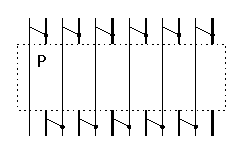
\includegraphics[scale=1.5]{figuras/sheeranrecurrence.eps}
    \caption{Patrón de recurrencia}
    \label{sheeranrecurrence}
 \end{subfigure}
 \begin{subfigure}{0.4\textwidth}
    \centering
    \includegraphics[scale 1.4]{figuras/wrapR.eps}
    \caption{Primeras iteraciones de ppNet}
    \label{firstsiter}
 \end{subfigure}
 \caption{Construcción de la red de prefijos paralelos}
\end{figure}


La figura \ref{firstsiter} representa las dos primeras iteraciones del circuito \verb|ppNet|, en el cual la caja de lineas punteada es el caso base de la descripción, los puntos negros son la función \verb|dotOp|. Lo que producimos con esta función recursiva son redes como la de la figura \ref{bKung16}.

A continuación, describimos el circuito \verb|ppNet|, pero antes escribimos las funciones auxiliares \verb|dop|, \verb|unzipl|, \verb|zipl|, \verb|comb|, \verb|posComb|, \verb|miti| y \verb|wrap|, que nos servirán para escribir \verb|ppNet|:


%abss era abs, pero lo renombré xq latex lo resaltaba como una función.
\begin{lstlisting}
dop [a, b] = [a, dotOp(a, b)]
--
unzipl []        = ([],[])
unzipl [a]       = ([a], [])
unzipl (a:b:abss) = (a:as, b:bs)
   where
      (as, bs) = unzipl abss
--
zipl ([], [])     = []
zipl ([a], [])    = []
zipl (a:as, b:bs) = a:b:zipl(as, bs)
--
-- La forma en que hemos escrito las funciones zipl y unzipl 
-- son la clave para lograr una descripcion de un sumador 
-- binario que acepte cualquier cantidad de entradas
--
comb []     = []
comb [a]    = []
comb (a:as) = dop [a, head as] ++ comb (tail as)
--
posComb (a:as)  = a: (comb (init as))++ [last as]
--
miti p = unzipl ->- (id -|- p) ->- zipl
--
wrap p = comb ->- miti p ->- posComb 
\end{lstlisting}

\noindent Luego finalemente, podemos describir {\verb|ppNet|}:

\begin{lstlisting}
ppNet [a]    = []
ppNet [a, b] = dop [a, b]
ppNet as     = wrap ppNet as
\end{lstlisting}


\subsubsection{Circuito top level}
Ahora que ya tenemos construidas todas las partes del sumador, sólo resta juntarlas siguiendo el esquemático de la figura \ref{bkungadder}. Prestar atención a que el circuito \verb|fork| realiza una copia de las señales, el \verb|even| deja pasar los bits pares, \verb|odd| los impares, \verb|id| es la función identidad y \verb|sums| mapea los bits de entrada con la función booleana XOR, salvo el primer y último bit:

\begin{lstlisting}
fork as = (as, as)
--
even as = cs
   where
      (bs,cs) = unzip as
--
odd as = bs
   where
      (bs,cs) = unzip as
-- Unas definiciones mas cortas:
dropP = id -|- odds
dropG = even -|- ppNet
--
sums (a:as,bs) = (a:lastXor (as,init bs),cOut)
   where
      cOut = last bs
--
lastXor (as, bs) = map xor2 cs
   where
      cs = zipp (as, bs)
--
zipp ([],[]) = []

zipp (a:as, b:bs) = c:cs  -- da lo mismo que poner (c:cs)
   where
      c  = (a, b)
      cs = zipp (as, bs)
\end{lstlisting}

\noindent Y el circuito completo es:
\begin{lstlisting}
fastAdd = gAndPs ->- fork ->- dropG ->- dropP ->- sums
\end{lstlisting}

\subsection{Simulación}
En Lava podemos simular el circuito usando la operación {\footnotesize\verb.simulate.}, el circuito y el estado de las entradas, por ejemplo:

{\footnotesize
\begin{verbatim}
simulate fastAdd ([high,low],[low,high])
\end{verbatim}
}

\noindent devuelve:{\footnotesize \verb|([high,high],low)|}. También podemos simular secuencia de entradas con la operación {\footnotesize\verb|simulateSeq|}:

{\footnotesize
\begin{verbatim} 
simulateSeq halfAdd [(low,low),(high,low),(low,high)]
\end{verbatim}
}

\noindent que devuelve {\footnotesize\verb|[(low,low),(high,low),(high,low)]|}

\subsubsection{Simulaciones con números decimales}
Lava nos permite una interfase con números enteros, por si nos interesa simular usando como operandos números enteros. Esto lo logramos si definimos una función como la siguiente, que toma dos enteros y convierte el segundo en un número binario de la cantidad de bits que indica el primero:
\begin{lstlisting}
int2bin 0 num = []

int2bin n num = (bit:bits)
  where
    (bit, num') = numBreak num
     bits      = int2bin (n-1) num'
\end{lstlisting}

\subsubsection{Método de validación del hardware}
Para este diseño en particular, no utilizaremos la simulación como una forma de validar el correcto funcionamiento del circuito, por eso no avanzaremos en las distintas alternativas de simulación que nos permite el sistema, como puede ser la creación de un archivo VCD\footnote{VCD: Value Change Dump es un formato basado en ASCII para loguear señales, que es utilizado por herramietas de simulación lógica. Para visualizarlo podemos utilizar el software GTKWave, de licencia libre.} a partir de vectores de entrada\footnote{Podemos usar una libreria de Haskell llamada \emph{casualmente} vcd que nos permite escribir y leer archivos con este formato}.

Justificamos descartar la simulación como método de validación por la simple razón de que sólo simulando todos los posibles estados de las entradas se garantiza el correcto diseño del circuito. Por ejemplo, para un sumador de 64 bits, es necesario simular $2^{128}$ estados.

Para este tipo de sistemas es aplicable la verificación formal automática, que desarrollaremos en el capítulo \ref{verificacion}.

\subsection{Síntesis del Netlist VHDL}

Para continuar en nuestro flujo de diseño, precisamos generar el circuito en un lenguaje que nuestra herramienta de \emph{Place and Route} pueda manejar. Para eso lava nos permite crear un netlist VHDL siguiendo dos pasos, el primero definiendo los nombres de los puertos y el bloque a ser creado:
\begin{lstlisting}
fastAdder n = writeVhdlInputOutputNoClk
              "BrentKungFastAdder" fastAdd
              (varList n "a", varList n "b")
              (varList n "sum", var "cout")
\end{lstlisting}

Y el segundo paso para crear el netlist, debemos especificar el valor real de sumador, por lo tanto valuamos el circuito con en número de bits del sumador y conseguiremos el archivo BrentKungFastAdder.vhl que mostramos en el apéndice \ref{vhdlNetlist}:
\begin{lstlisting}
Main> fastAdder 16
Writing to file "BrentKungFastAdder.vhd" ... Done..
\end{lstlisting}

\noindent Si por alguna razón este netlist lo utilizaramos con una otra herramienta de síntesis, deberemos especificar que no modifique los cables para preservar la estructura de esta red.

